\noindent A terceira função escolhida foi \(f_3(x) = cos(x) - x\). O código implementado para construção do gráfico e da tabela é semelhante aos das funções anteriores:

\lstinputlisting{II/f3.m}
O gráfico e a tabela obtidos são os seguintes:

\begin{figure}[ht]
    \centering
    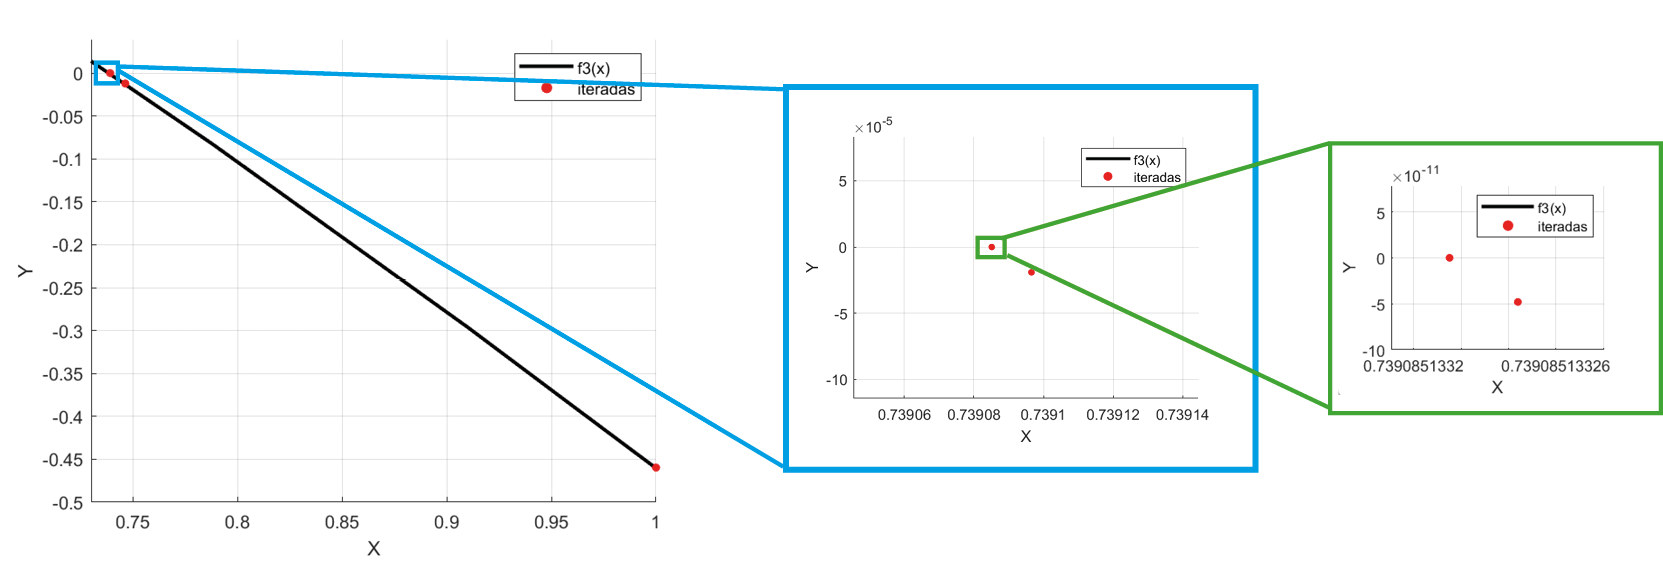
\includegraphics[width=\textwidth]{II/grafico_f3.png}
    \label{grafico_f3}
\end{figure}

\begin{table}[ht]
    \centering
    \begin{tabular}{|c|c|c|c|c|c|}
    \hline
    \(n\) & \(x_n\) & \(|e_n|\) & \(\displaystyle \frac{|e_{n+1}|}{|e_n|}\) & \(\displaystyle \frac{|e_{n+1}|}{|e_n|^2}\) & \(\displaystyle \frac{|e_{n+1}|}{|e_n|^3}\) \\
    \hline
    0 & $1.000000000000000$ & $0.260914$                 & $0.027744$                & $0.106335$ & $0.407548$ \\
    1 & $0.746324095080226$ & $0.007238$                 & $0.001576$                & $0.217764$ & $30.08226$ \\
    2 & $0.739096544625631$ & $1.141141 \times 10^{-5}$  & $2.519641 \times 10^{-6}$ & $0.220800$ & $1.934907 \times 10^4$ \\
    3 & $0.739085133243913$ & $2.875266 \times 10^{-11}$ & & & \\
    4 & $0.739085133215161$ & & & & \\
    \hline
    \multicolumn{6}{|c|}{$p = 2\quad K_{\infty} \approx 0.2$}\\
    \hline
    \end{tabular}
\end{table}

\noindent Pelo gráfico percebe-se que, de facto, as iteradas estão a convergir para \(z\). Os valores da tabela permitem concluir que \(\displaystyle \frac{|e_{n+1}|}{|e_n|}\) deve convergir para 0 e \(\displaystyle \frac{|e_{n+1}|}{|e_n|^3}\) deve convergir para \(\infty\). Já os valores \(\displaystyle \frac{|e_{n+1}|}{|e_n|^2}\) devem convergir para um \(K_\infty \approx 0.2\), mostrando a convergência de ordem 2.